\documentclass{standalone}
\usepackage{tikz}
\usetikzlibrary{datavisualization}
\usepackage[range-phrase = --,retain-unity-mantissa = false,exponent-product = \cdot]{siunitx}

\begin{document}
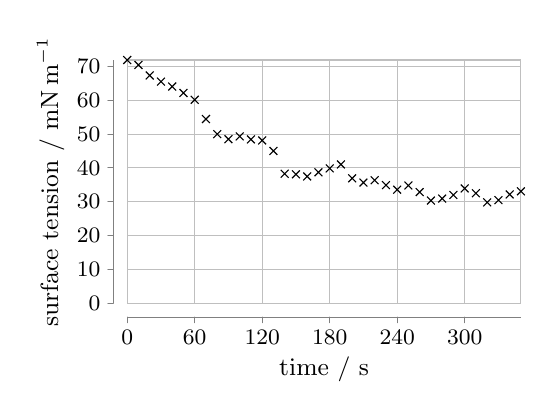
\begin{tikzpicture}
  \datavisualization [ scientific axes=clean,
  x axis={attribute=time, grid, ticks={step=60}, label={time / \si{\second}}},
  y axis={attribute=surface tension, include value=0, grid,
    label={surface tension / \si{\milli\newton\per\metre}}},
  style sheet=strong colors,
  visualize as scatter ]
  % data [read from file=Surfactine_954_2015-07-13-3.csv] ;
  data {
    time, capillary length, surface tension
    0, 2.71, 71.87
    10, 2.68, 70.41
    20, 2.62, 67.3
    30, 2.58, 65.5
    40, 2.55, 64.04
    50, 2.52, 62.13
    60, 2.48, 60.13
    70, 2.36, 54.44
    80, 2.26, 49.97
    90, 2.22, 48.48
    100, 2.24, 49.31
    110, 2.22, 48.41
    120, 2.21, 48.11
    130, 2.14, 45.01
    140, 1.98, 38.27
    150, 1.97, 38.11
    160, 1.95, 37.47
    170, 1.99, 38.7
    180, 2.02, 39.86
    190, 2.04, 41.02
    200, 1.96, 36.92
    210, 1.91, 35.67
    220, 1.93, 36.36
    230, 1.89, 34.92
    240, 1.85, 33.56
    250, 1.88, 34.81
    260, 1.83, 32.86
    270, 1.76, 30.36
    280, 1.78, 30.94
    290, 1.81, 32.0
    300, 1.86, 33.93
    310, 1.82, 32.52
    320, 1.74, 29.82
    330, 1.76, 30.48
    340, 1.81, 32.16
    350, 1.84, 33.08
  };
\end{tikzpicture}
\end{document}
